% a-project.tex, v-1.0.3 marcoreis baseado no
% abntex2-modelo-trabalho-academico.tex, v-1.9.7 laurocesar
% Copyright 2012-2018 by abnTeX2 group at http://www.abntex.net.br/ 
% 
% This work consists of the files ........
% 
% -----------------------------------------------------------------------------
% Modelo para desenvolvimento de documentação de projetos acadêmicos
% (tese de doutorado, dissertação de mestrado e trabalhos de monografias em geral) 
% em conformidade com ABNT NBR 14724:2011: Informação e documentação. 
% -----------------------------------------------------------------------------
% Opções para a documentação
%
% Fancy page headings 
%\documentclass[fancyheadings, subook]{Classes/a-prj}
%\documentclass[fancyheadings, sureport]{Classes/a-prj}
%
% Fancy chapters and sections headings 
%\documentclass[fancychapter, subook]{Classes/a-prj}
%\documentclass[fancychapter, sureport]{Classes/a-prj}
%
% Fancy page , chapters and sections headings
%\documentclass[fancyheadings, fancychapter, subook]{Classes/a-prj}
\documentclass[fancyheadings, fancychapter, sureport]{Classes/a-report}
%
% -----------------------------------------------------------------------------
% Alguns comandos para a fancy page headings)
%
% Page header line width
%\footlinewidth{value}
%
% Page footer line width
%\headlinewidth{value}
%
% Page header and footer line width
%\headingslinewidth{value}
%
% Page header and footer lines without text
%\headingslinesonly
%
% The default line width is 0.3pt.
% Set the value to 0pt to remove the page header and/or footer line
%
% -------------------------------------------------------------------------------
% Formato de figuras suportado
% -------------------------------------------------------------------------------
% O formato das figuras depende da forma como o arquivo de saída é gerado.
% As figuras inseridas na pasta Figures serão automaticamente reconhecidas sem
% a necessidade de inserir a extensão do arquivo.
%
% O pdfLaTEX (PDF) suporta figuras com as extensões: pdf, jpg, png e mps.
%
% -------------------------------------------------------------------------------
% Árvore do diretório a-project.tex
%  Diretório
%       \Classes        (requerido)
%       \Figures        (requerido) --------------------------------->
%       \Figures\PDF    (optional)
%       \Figures\JPG    (optional) Figures located within these
%       \Figures\PNG    (optional) folders are searched automatically
%       \Figures\MPS    (optional)  by the a-prj class.
%       \Figures\EPS    (optional)
%       \Figures\PS     (optional) <--------------------------------
%       \Tables         (requerido)
%       \Others         (requerido)
%       \Chapters       (requerido)
%       \Appendices     (optional)
%       \References     (requerido)
%
% -------------------------------------------------------------------------------
% PDF File resumo
\ifpdf
    \hypersetup{
    	backref,
        colorlinks  = true,
        pdftitle    = Modelo de documentação,
        pdfauthor   = {Marco Reis, marco.a.reis@gmail.com},
        pdfsubject  = Mestre em Engenharia,
        pdfcreator  = Subtitulo,
        pdfproducer = PDFLatex,
        pdfkeywords = {documentação, latex, dissertação, tese}}
 \fi
%
% -------------------------------------------------------------------------------
% Relação de pacotes opcionais utilizados
\usepackage[utf8]{inputenc}
\usepackage[brazil]{babel}
\usepackage{longtable}
\usepackage{dcolumn}
\usepackage{multirow}
\usepackage{lscape}
%\usepackage{graphicx}
\usepackage{rotating}
%\usepackage{float,subfigure}
%\usepackage{graphicx, subfigure}
\usepackage{cite}
\usepackage[left=3cm,top=3cm,right=2cm,bottom=2cm]{geometry}
\usepackage[alf]{abntex2cite}
\usepackage{ifpdf}
\usepackage{shadow}
\usepackage{wrapfig}
\usepackage[normalem]{ulem}
\usepackage{makeidx}
\usepackage{yfonts}
\usepackage{algorithm}
\usepackage{algorithmic}
\usepackage{lmodern}
\usepackage[T1]{fontenc}
\usepackage{indentfirst}
\usepackage{color}
\usepackage{microtype}
\usepackage{lipsum}
\usepackage{caption}
\usepackage{subcaption}
%
\makeindex 
\setlength{\LTcapwidth}{\textwidth}
%
\newtheorem{theorem}{Teorema}
\newtheorem{definition}[theorem]{Definição}
%
% -------------------------------------------------------------------------------
% Configurações do pacote backref
\renewcommand{\backrefpagesname}{Citado na(s) página(s):~}
% Texto padrão antes do número das páginas
\renewcommand{\backref}{}
% Define os textos da citação
\renewcommand*{\backrefalt}[4]{
	\ifcase #1 %
		Nenhuma citação no texto.%
	\or
		Citado na página #2.%
	\else
		Citado #1 vezes nas páginas #2.%
	\fi
}
% 
% -------------------------------------------------------------------------------
% Início do documento raiz
\begin{document}
% Definição do título da página
    \university{Centro Universitário SENAI CIMATEC}
	%\faculty{Programa de...}
	%\school{Escola de...}
% 
    %\course{Engenharia Elétrica}
    \typework{Relatório Final}
% 
	%\course{Mestrado em Modelagem Computacional e Tecnologia Industrial}
	%\typework{Disserta\c{c}\~ao de mestrado}
	%\typework{Exame de Qualificação de Mestrado}
% 
	%\course{Engenharia Elétrica}
	%\typework{Tese de doutorado}
	%\typework{Exame de Qualificação de doutorado}
%
% -------------------------------------------------------------------------------
% Informações gerais
    \thesistitle{Implementação do Planejador\\ Probabilistic Roadmap}
    \hidevolume
    \thesisvolume{Volume 1 of 1}
    \thesisauthor{Mateus Zarth Seixas}
    % \thesisauthorr{Rick Deckard}
    \thesisadvisor{Prof. Marco Reis, M.Eng.}
    %\hidecoadvisor
    %\thesiscoadvisor{Marco Reis}
    \thesismonthyear{Dezembro de 2021}
% 
    \maketitlepage
%
% ----------------------------------------------------------------------------
% Inserir Folha de rosto, Nota de estilo, folha de assinaturas, dedicatoria
    \begin{folharosto}

\begin{center}
\theauthor \\
% \theauthorr \\
%\theauthorrr \\
%\theauthorrrr \\
%\theauthorrrrr \\
\end{center}
\ \\
\ \\
\ \\
\ \\
\ \\
\begin{spacing}{2}
   \begin{center}
   {\LARGE {\bf \thetitle}}
   \end{center}
\end{spacing}
\ \\
\ \\
\ \\
\vspace*{85mm}
% \begin{flushright}

%    \begin{list}{}{
%       \setlength{\leftmargin}{7.5cm}
%       \setlength{\rightmargin}{0cm}
%       \setlength{\labelwidth}{0pt}
%       \setlength{\labelsep}{\leftmargin}}

%       \item \thetypework apresentada ao \thefaculty, Curso de \thecourse
%       do \theuniversity, como requisito parcial para a obten\c{c}\~ao do
%       t\'itulo de {\bf \thedegreetitle}.

%       \begin{list}{}{
%       \setlength{\leftmargin}{0cm}
%       \setlength{\rightmargin}{0cm}
%       \setlength{\labelwidth}{0pt}
%       \setlength{\labelsep}{\leftmargin}}

%       \item \'Area de conhecimento: Interdisciplinar

%       \item Orientador: \theadvisor
%       \newline \hspace*{2.1cm}  %{\it \theuniversity}

%       \end{list}
%    \end{list}

% \end{flushright}
\ \\
\ \\
\ \\
\ \\
%\begin{spacing}{1.5}
   \begin{center}
   Salvador \par
   \theuniversity \par
   2020
   \end{center}
%\end{spacing}

\end{folharosto}

    %\begin{notaestilo}
Esta \thetypeworkthree foi elaborada considerando as normas de
estilo (i.e. est\'eticas e estruturais) propostas aprovadas pelo
colegiado do \thefacultytwo e est\~ao dispon\'iveis em formato
eletr\^onico ({\it download} na P\'agina Web
http:$//$ead.fieb.org.br$/$portal\_faculdades$/$dissertacoes-e-teses-mcti.html
ou solicita\c{c}\~ao via e-mail \`a secretaria do
programa) e em formato impresso somente para consulta. \\

Ressalta-se que o formato proposto considera diversos itens das
normas da Associa\c{c}\~ao Brasileira de Normas T\'ecnicas (ABNT),
entretanto opta-se, em alguns aspectos, seguir um estilo pr\'oprio
elaborado e amadurecido pelos professores do programa de
p\'os-gradua\c{c}\~ao supracitado.

\end{notaestilo}

    %\begin{folhaassinaturas}

%\thispagestyle{empty}

\def\signature#1#2{\parbox[b]{1in}{\smash{#1}\vskip12pt}
\hfill \parbox[t]{3in}{\shortstack{\vrule width 3in height
0.4pt\\\small#2}}}

\def\InstituicaoMembro#1#2{\parbox[b]{1in}{\smash{#1}\vskip12pt}
\hfill \parbox[t]{3in}{\shortstack{\vrule width 3in \\\small#2}}}

\def\signaturepage{%

    \begin{spacing}{1.5}
        \begin{center}
        {\LARGE \theuniversity} \\
        {\large \thefaculty} \\
        {\large \thecourse} \\
        \end{center}
    \end{spacing}

   \vskip 0.25in plus 0.4in minus 0.1in

    \begin{spacing}{1.5}
        \begin{sloppypar}
        A Banca Examinadora, constitu\'ida pelos professores abaixo
        listados, leram e recomendam a aprova\c{c}\~ao [com distin\c{c}\~ao] da
        \thetypeworktwo, intitulada ``\thetitle",
        apresentada no dia (dia) de (m\^es) de (ano), como requisito
        parcial para a obten\c{c}\~ao do t\'itulo de {\bf \thedegreetitle}.\\
        \end{sloppypar}
    \end{spacing}

    \def\sigskip{\vskip0.15in plus 0.2in minus 0.1in}
    \def\beginskip{\vskip0.3875in plus 0.2in minus 0.1in}

    \beginskip
    \signature{Orientador:}{Prof. Dr. \theadvisor} \\
    \InstituicaoMembro{}{\theuniversity} \\

    \sigskip
    \beginskip
    \signature{Membro externo da Banca:}{Prof. Dr. Nome completo} \\
    \InstituicaoMembro{}{Institui\c{c}\~ao do membro da banca} \\

    \sigskip
    \beginskip
    \signature{Membro externo da Banca:}{Prof. Dr. Nome completo} \\
    \InstituicaoMembro{}{Institui\c{c}\~ao do membro da banca} \\

    %\sigskip
    %\beginskip
   % \signature{Membro interno da Banca:}{Prof. Dr. Nome completo} \\
   % \InstituicaoMembro{}{Institui��o do membro da banca} \\

    \vfill
    \newpage
    \setcounter{page}{3}
}
%*********************************************************************


\signaturepage


\end{folhaassinaturas}

    %\include{Others/dedicatoria}
    %\include{Others/agradecimentos}
%
% ----------------------------------------------------------------------------
% Resumo/abstract, sumário e siglas
    \begin{romanpagenumbers}
        % \begin{thesisresumo}
Escreva aqui o resumo da disserta\c{c}\~ao, incluindo os contextos geral e espec\'ifico, dentro dos quais a pesquisa foi realizada, o objetivo da pesquisa, assun\c{c}\~ao filos\'ofica, os m\'etodos de pesquisa usados e as poss\'iveis contribui\c{c}\~oes que o que \'e proposto pode trazer \`a sociedade.

\ \\

% use de três a cinco palavras-chave

\textbf{Palavras-chave}: Palavra-chave 1, Palavra-chave 2, Palavra-chave 3, Palavra-chave 4, Palavra-chave 5

\end{thesisresumo}

        % \begin{thesisabastract}
Escreva aqui, em ingl\^es, o resumo da disserta\c{c}\~ao, incluindo os contextos geral e espec\'ifico, dentro dos quais a pesquisa foi realizada, o objetivo da pesquisa, assun\c{c}\~ao filos\'ofica, os m\'etodos de pesquisa usados e as poss\'iveis contribui\c{c}\~oes que o que \'e proposto pode trazer \`a sociedade. 

\ \\

% use de tr�s a cinco palavras-chave

\textbf{Keywords}: Keyword 1, Keyword 2, Keyword 3, Keyword 4, Keyword 5

\end{thesisabastract}

        % Make list of contents, tables and figures
        \thesiscontents
        \pdfbookmark[1]{Lista de Tabelas}{lot} \listoftables
        \newpage
        %Include other required section
        %\begin{thesisabbreviations}
\begin{footnotesize}
\begin{longtable}[l]{p{2cm}l}
  tprax   \dotfill & \thefaculty \\
  WWW       \dotfill &  World Wide Web \\
\end{longtable}
\end{footnotesize}
\end{thesisabbreviations}

        %\begin{thesissymbols}
\begin{footnotesize}
\begin{longtable}[l]{p{2cm}l}
  $\partial$   \dotfill  & Bla bla bla \\
  $\prod$       \dotfill & ble ble ble \\
  $\partial$   \dotfill  & Bla bla bla \\
  $\prod$       \dotfill & ble ble ble \\
  $\partial$   \dotfill  & Bla bla bla \\
  $\prod$       \dotfill & ble ble ble \\
  $\partial$   \dotfill  & Bla bla bla \\
  $\prod$       \dotfill & ble ble ble \\
  $\partial$   \dotfill  & Bla bla bla \\
  $\prod$       \dotfill & ble ble ble \\
  $\partial$   \dotfill  & Bla bla bla \\
  $\prod$       \dotfill & ble ble ble \\
  $\partial$   \dotfill  & Bla bla bla \\
  $\prod$       \dotfill & ble ble ble \\
  $\partial$   \dotfill  & Bla bla bla \\
  $\prod$       \dotfill & ble ble ble \\
  $\partial$   \dotfill  & Bla bla bla \\
  $\prod$       \dotfill & ble ble ble \\
  $\partial$   \dotfill  & Bla bla bla \\
  $\prod$       \dotfill & ble ble ble \\
  $\partial$   \dotfill  & Bla bla bla \\
  $\prod$       \dotfill & ble ble ble \\
  $\partial$   \dotfill  & Bla bla bla \\
  $\prod$       \dotfill & ble ble ble \\
  $\partial$   \dotfill  & Bla bla bla \\
  $\prod$       \dotfill & ble ble ble \\
  $\partial$   \dotfill  & Bla bla bla \\
  $\prod$       \dotfill & ble ble ble \\
  $\partial$   \dotfill  & Bla bla bla \\
  $\prod$       \dotfill & ble ble ble \\
  $\partial$   \dotfill  & Bla bla bla \\
  $\prod$       \dotfill & ble ble ble \\
  $\partial$   \dotfill  & Bla bla bla \\
  $\prod$       \dotfill & ble ble ble \\
  $\partial$   \dotfill  & Bla bla bla \\
  $\prod$       \dotfill & ble ble ble \\
  $\partial$   \dotfill  & Bla bla bla \\
  $\prod$       \dotfill & ble ble ble \\          
\end{longtable}
\end{footnotesize}
\end{thesissymbols}

        %Switch the page numbering back to the default format
    \end{romanpagenumbers}
%
% ---------------------------------------------------------------------------
% Include thesis chapters
    \parskip=\baselineskip
    \chapter{Introdução}
\label{chap:intro}

Nesse estudo foi feita a implementação do algoritmo de planejamento de trajetória Probabilistic Roadmap (PRM) em um robô diferencial não-holonômico chamado Turtlebot3 para permitir a navegação autônoma desse robô. Os testes foram realizados em ambiente de simulação e em um labirinto real construído. 

\begin{figure} [h!]	
  \centering
  \caption{Turtlebot3}
  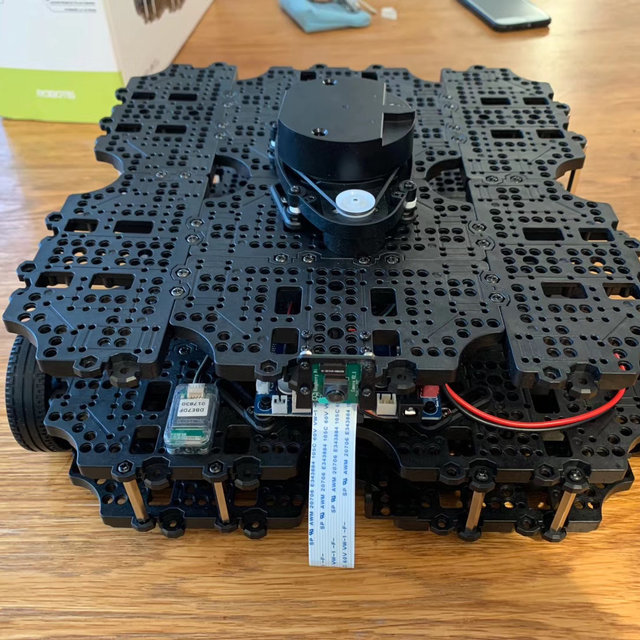
\includegraphics[width=0.6\textwidth,trim={0 1.5cm 0 1.5cm},clip]{Figures/TurtleBot3-Waffle-Pi-robotic-platform_Q640.jpg}
  \caption*{Fonte: Autoria própria.}
  \label{fig:turt1}
\end{figure}

%--------- NEW SECTION ----------------------
\section{Objetivos}
\label{sec:obj}
O objetivo desse estudo foi fazer a implementação do algoritmo de planejamento de trajetória PRM no Turtlebot3 para ser integrada à navegação desse robô como planejador global, a fim de que esse robô pudesse ser capaz de navegar autonomamente em um labirinto, após mapeado, indo de um ponto a outro sem colidir com os obstáculos.
\label{sec:obj}

%--------- NEW SECTION ----------------------
\section{Justificativa}
\label{sec:justi}

Em um trabalho futuro, o algoritmo de planejamento aqui desenvolvido será comparado com outras técnicas de planejamento e trajetória, como A*, D* e Dijkstra, para comparar seus resultados estatisticamente.

%--------- NEW SECTION ----------------------
\section{Organização do documento}
\label{section:organizacao}

Este documento apresenta $5$ capítulos e está estruturado da seguinte forma:

\begin{itemize}

  \item \textbf{Capítulo \ref{chap:intro} - Introdução}: É apresentado o estudo realizado, com a descrição do problema, objetivo e justificativa.;
  \item \textbf{Capítulo \ref{chap:fundteor} - Fundamentação Teórica}: É apresentada a base teórica que sustenta o estudo desenvolvido;
  \item \textbf{Capítulo \ref{chap:metod} - Materiais e Métodos}: XXX;
  \item \textbf{Capítulo \ref{chap:result} - Resultados}: XXX;
  \item \textbf{Capítulo \ref{chap:conc} - Conclusão}: Apresenta as conclusóes, contribuições e algumas sugestões de atividades de pesquisa a serem desenvolvidas no futuro.

\end{itemize}

    \chapter{Fundamentação Teórica}
\label{chap:fundteor}
%--------- NEW SECTION ----------------------

O estudo tinha como objetivo fazer a implementação do planejador de trajetória PRM no robô diferencial Turtlebot3. Nesse capítulo serão apresentadas as características do robô e do planejador de trajetória Probabilistic Roadmap.

%conferir se precisa de requisitos do cliente
\section{Turtlebot3}
O Turtlebot3 é um robô diferencial não-holonômico desenvolvido pela empresa Robotis e tem como o ambiente de desenvolvimento padrão o ROS (Robot Operating System). O Turtlebot3 tem como unidade central de processamento uma Raspberry Pi e o sistema operacional instalado nela foi o Ubuntu 20.04 com o ROS Noetic. 

O Turtlebot3 tem 2 modelos, o Burger e o Waffle Pi. O modelo escolhido para esse desenvolvimento foi o Waffle Pi, que conta o motor DYNAMIXEL (XM430-W210-T) e uma câmera Raspberry Pi, componentes que o diferenciam do modelo Burger, além do seu formato. O Turtlebot3 conta com um sensor de escaneamento a laser LiDar, uma OpenCR, módulo Bluetooth e uma beteria Li-Po. Pode-se ver o robô e seus componentes na Figura \ref{fig:turt2}.

\begin{figure} [h!]	
   \centering
   \caption{Turtlebot3 e seus Componentes}
   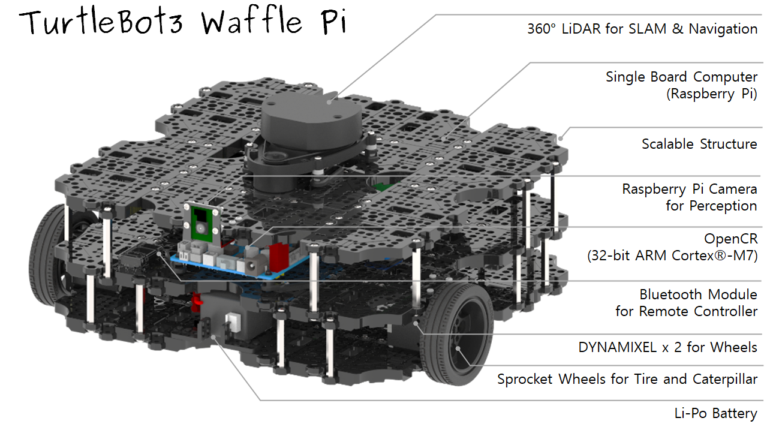
\includegraphics[width=0.8\textwidth]{Figures/turtlebot3_waffle_pi_components.png}
   \caption*{Fonte: Autoria própria.}
   \label{fig:turt2}
\end{figure}

\section{Probabilistic Roadmap}

O algoritmo Probabilistic Roadmap é um planejador de trajetória que permite que um robô se desloque de um ponto inicial a um ponto final sem a interferência de um operador evitando a colisão com obstáculos. A ideia do planejador é gerar pontos aleatórios no mapa, verificando se esses pontos são espaços livres ou não, e tentando conectar eles com os outros pontos mais próximos já gerados, caso não tenha nenhuma barreira entre esses pontos. A medida que o número de pontos cresce, vão se formando trajetórias entre todos os espaços livres do mapa, como mostrado na Figura \ref{fig:prm}.

\begin{figure} [h!]	
   \centering
   \caption{Probabilistic Roadmap}
   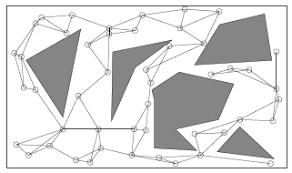
\includegraphics[width=0.6\textwidth]{Figures/images.png}
   \caption*{Fonte: Autoria própria.}
   \label{fig:prm}
\end{figure}

O algoritmo PRM tem duas fases, uma fase de construção do mapa de rotas e uma fase de questionamento. Na fase de construção, são gerados nós em pontos aleatórios do mapa que estejam em espaços livres. Cada nó desse é então ligado a número k de nós mais próximos, verificando se não a colisão no caminho. O mapa de rotas é construído então de maneira incremental e armazenado.

Na fase de questionamento, são declarados no algoritmo o ponto inicial e o ponto final do robô, sendo utilizado alguma técnica para calcular o caminho de menor custo. O algoritmo utilizado nesse caso foi o A*.

\section{Move Base}

O pacote de navegação para ROS utilizado para auxiliar nessa funcionalidade do robô é o Move Base. Através dele é possível declarar uma ação para o robô se deslocar de uma posição inicial para um posição final utilizando um planejador global e um planejador local. Nesse estudo o planejador global que será utilizado é o planejador de trajetória PRM. Na Figura \ref{fig:move} é possível ver um esquemático de como o Move Base funciona

\begin{figure} [h!]	
   \centering
   \caption{Move Base}
   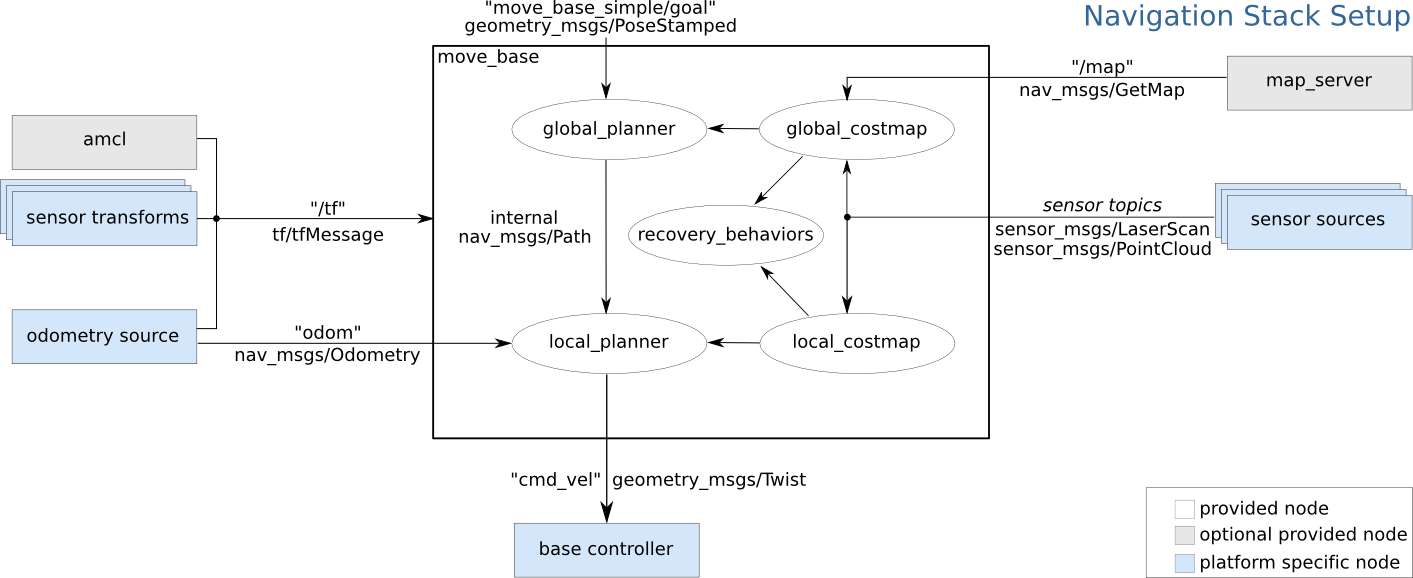
\includegraphics[width=1\textwidth]{Figures/overview_tf.png}
   \caption*{Fonte: Autoria própria.}
   \label{fig:move}
\end{figure}
    \chapter{Desenvolvimento do projeto}
\label{chap:metod}
Nesta seção será descrito o procedimento utilizado para construção inicial do robô Walker, incluindo as fases conceitual e design.  Será apresentado a ideação do projeto, especificações e as funcionalidades.

\section{Ideação}
%escrever oq sera apresentado

\subsection{Arquitetura Geral}
 A arquitetura geral, apresentada na Figura \ref{fig:Arquitetura geral}, relaciona de modo geral a interface do usuário, com a central de gerenciamento do sistema e com a interface com hardware. Neste contexto, a interface do usuário representa o contato direto com o usuário por meio de um botão \textit{on/off}, um \textit{joystick} e por acesso remoto, através de um computador devidamente conectado.

 \begin{figure} [h!]	
    \centering

    \caption{Arquitetura Geral}
    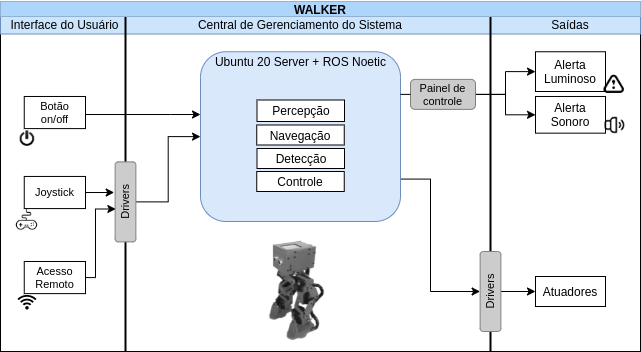
\includegraphics[width=0.8\textwidth]{general_architecture}
    \caption*{Fonte: Autoria própria.}
    \label{fig:Arquitetura geral}
\end{figure}	

Para a central de gerenciamento do sistema utilizou-se o sistema operacional \textit{Ubuntu} 20.04 junto ao framework de robótica ROS \textit{Noetic}. Neste cojunto se encontram as principais funcionalidades do robô: percepção, navegação, detecção e controle. Por fim, no conjunto de saídas estão os atuadores e os alertas sonoro e luminoso.

\subsection{Requisitos técnicos}

%desdobramento da função qualidade
\subsection{Quality Function Deployment}
\textit{Quality Function Deployment} é uma ferramenta de qualidade que auxilia na conversão das demandas do cliente em características de qualidade do produto. Dessa forma, no primeiro ciclo do QFD foram analisados os requisistos do cliente e os requisitos técnicos necessários, sinalizando os pontos mais importantes e as relações entre estes. O resultado foi exposto na \ref{fig:QFD}

\begin{figure} [h!]	
    \centering
    \caption{ Primeiro ciclo QFD}
    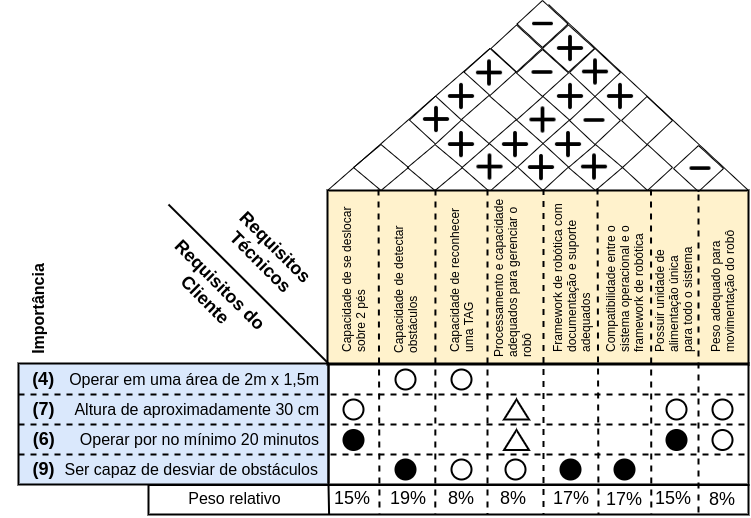
\includegraphics[width=0.8\textwidth]{Figures/QFD}
    \caption*{Fonte: Autoria própria.}
    \label{fig:QFD}
\end{figure}
 Através do QFD foi possível observar 

% %--------- NEW SECTION ----------------------
% \section{Interface do Usuário}
% \label{sec:ui}
% \lipsum[1]

% %--------- NEW SECTION ----------------------
% \section{Simulação do sistema}
% \label{sec:sim}
% \lipsum[2-4]


    \chapter{Resultados}
\label{chap:result}
Importante sempre ter um parágrafo introdutório para explicar os resultados encontrados.

%--------- NEW SECTION ----------------------
\section{Testes unitários}
\label{sec:testu}
\lipsum[1]

\section{Integração do sistema}
\label{sec:intsis}
\lipsum[1]

%--------- NEW SECTION ----------------------
\section{Testes integrados}
\label{sec:testi}
\lipsum[1]








    \chapter{Conclusão}
\label{chap:conc}

O estudo realizado trouxe maior entendimento sobre as funcionalidades de planejamento de trajetória e navegação, além de trazer conhecimento sobre o funcionamento do planejador Probabilistic Roadmap. Em ambiente de simulação o planejador teve bons resultados, porém na prática, para algumas trajetórias mais complicadas, o planejador não conseguiu obter solução, mas conseguiu lidar bem com trajetórias simples. Alguns parâmetros do move\textunderscore base podem ser ajustados para encontrar um melhor resultado da implementação do algoritmo. Para trabalhos futuros o serão implementadas os ajustes dos parâmetros e o resultado obtido com esse planejador será comparado com outros planejadores, como A*, D* e Dijkstra, para comparar seus resultados estatisticamente e ser
    % include more chapters ...
%
% ----------------------------------------------------------------------------
% Include thesis appendices
    \begin{thesisappendices}
        % % Thesis Appendix -------------------------------------------------------

\chapter{Diagramas mecânicos}
\label{Append:diagmec}



        % % Thesis Appendix -------------------------------------------------------

\chapter{Diagramas eletro-eletrônicos}
\label{Append:diagele}



        %% Thesis Appendix -------------------------------------------------------

\chapter{Logbook}
\label{Append:log}



    \end{thesisappendices}
%
% ----------------------------------------------------------------------------
% Configurar as referencias bibliograficas
	\renewcommand\bibname{Referências}
    \addcontentsline{toc}{chapter}{Referências}
    \bibliography{References/referencias}
%
% ----------------------------------------------------------------------------
% Finishing him
    \include{Others/ultimafolha}
\end{document}
%
% -------------------------------------------------------------------------------
% Aqui termina a formatação para o documento.
% In God We Trust. All Other Bring Data. 
%
% -------------------------------------------------------------------------------